
    \subsection*{Hierarchical Clustering}
    
        That last example reveals something: not all types of groups are the same! Some are much broader than others, for example.
        
        If two types of groups are different, then why do we only have to have one type in our clustering? We don't have to restrict ourselves to a single $k$.
        
        Instead, we could treat some groups as inside of other groups: we call this a \textit{hierarchy}, because some groups are "higher" on the scale.\\
        
        \begin{definition}
            \vocab{Hierarchical Clustering} is when we cluster at multiple different \purp{levels}. 
            
            Some groups are \vocab{high-level}, or \purp{coarse}: they are groupings that contains \gren{more elements}: items in the same group can be more \purp{different}.
            
            Some groups are \vocab{low-level}, or \purp{fine}: they are groupings that contain \gren{fewer elements}: items in the same group have to be very \purp{similar}.
        \end{definition}
        
        \miniex Categorizing living things is done using hierarchical clustering: some groupings \textbf{contain} other groupings.
        
        \begin{figure}[H]
            \centering
            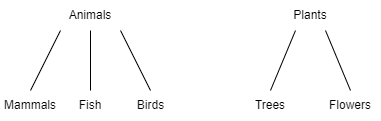
\includegraphics[width=70mm,scale=0.4]{images/clustering_images/hierarchical_life.png}
            \caption*{The top row of clusters are more \textbf{coarse}, while the bottom row is more \textbf{fine}.}
        \end{figure}
        
        We can \textbf{split} our groupings into \textbf{smaller} and smaller ones, to be as \textbf{fine-grained} as we need. Useful!
